\section{Cross check between Andrey Kim and Bobby Johnston}

As an additional cross check, Bobby calculated a $DV\pi^0P$ beam spin asymmetry and compared to Andrey Kim's results. This check will not comment on any acceptance, luminosity, or virtual photon flux factor calculations, but does validate exclusive event selection criteria. By examining figure \ref{fig:bsa} we can see that agreement is reasonable, especially considering Bobby's calculation does not have sideband subtraction included.

\begin{figure}[hbt]
	\centering
	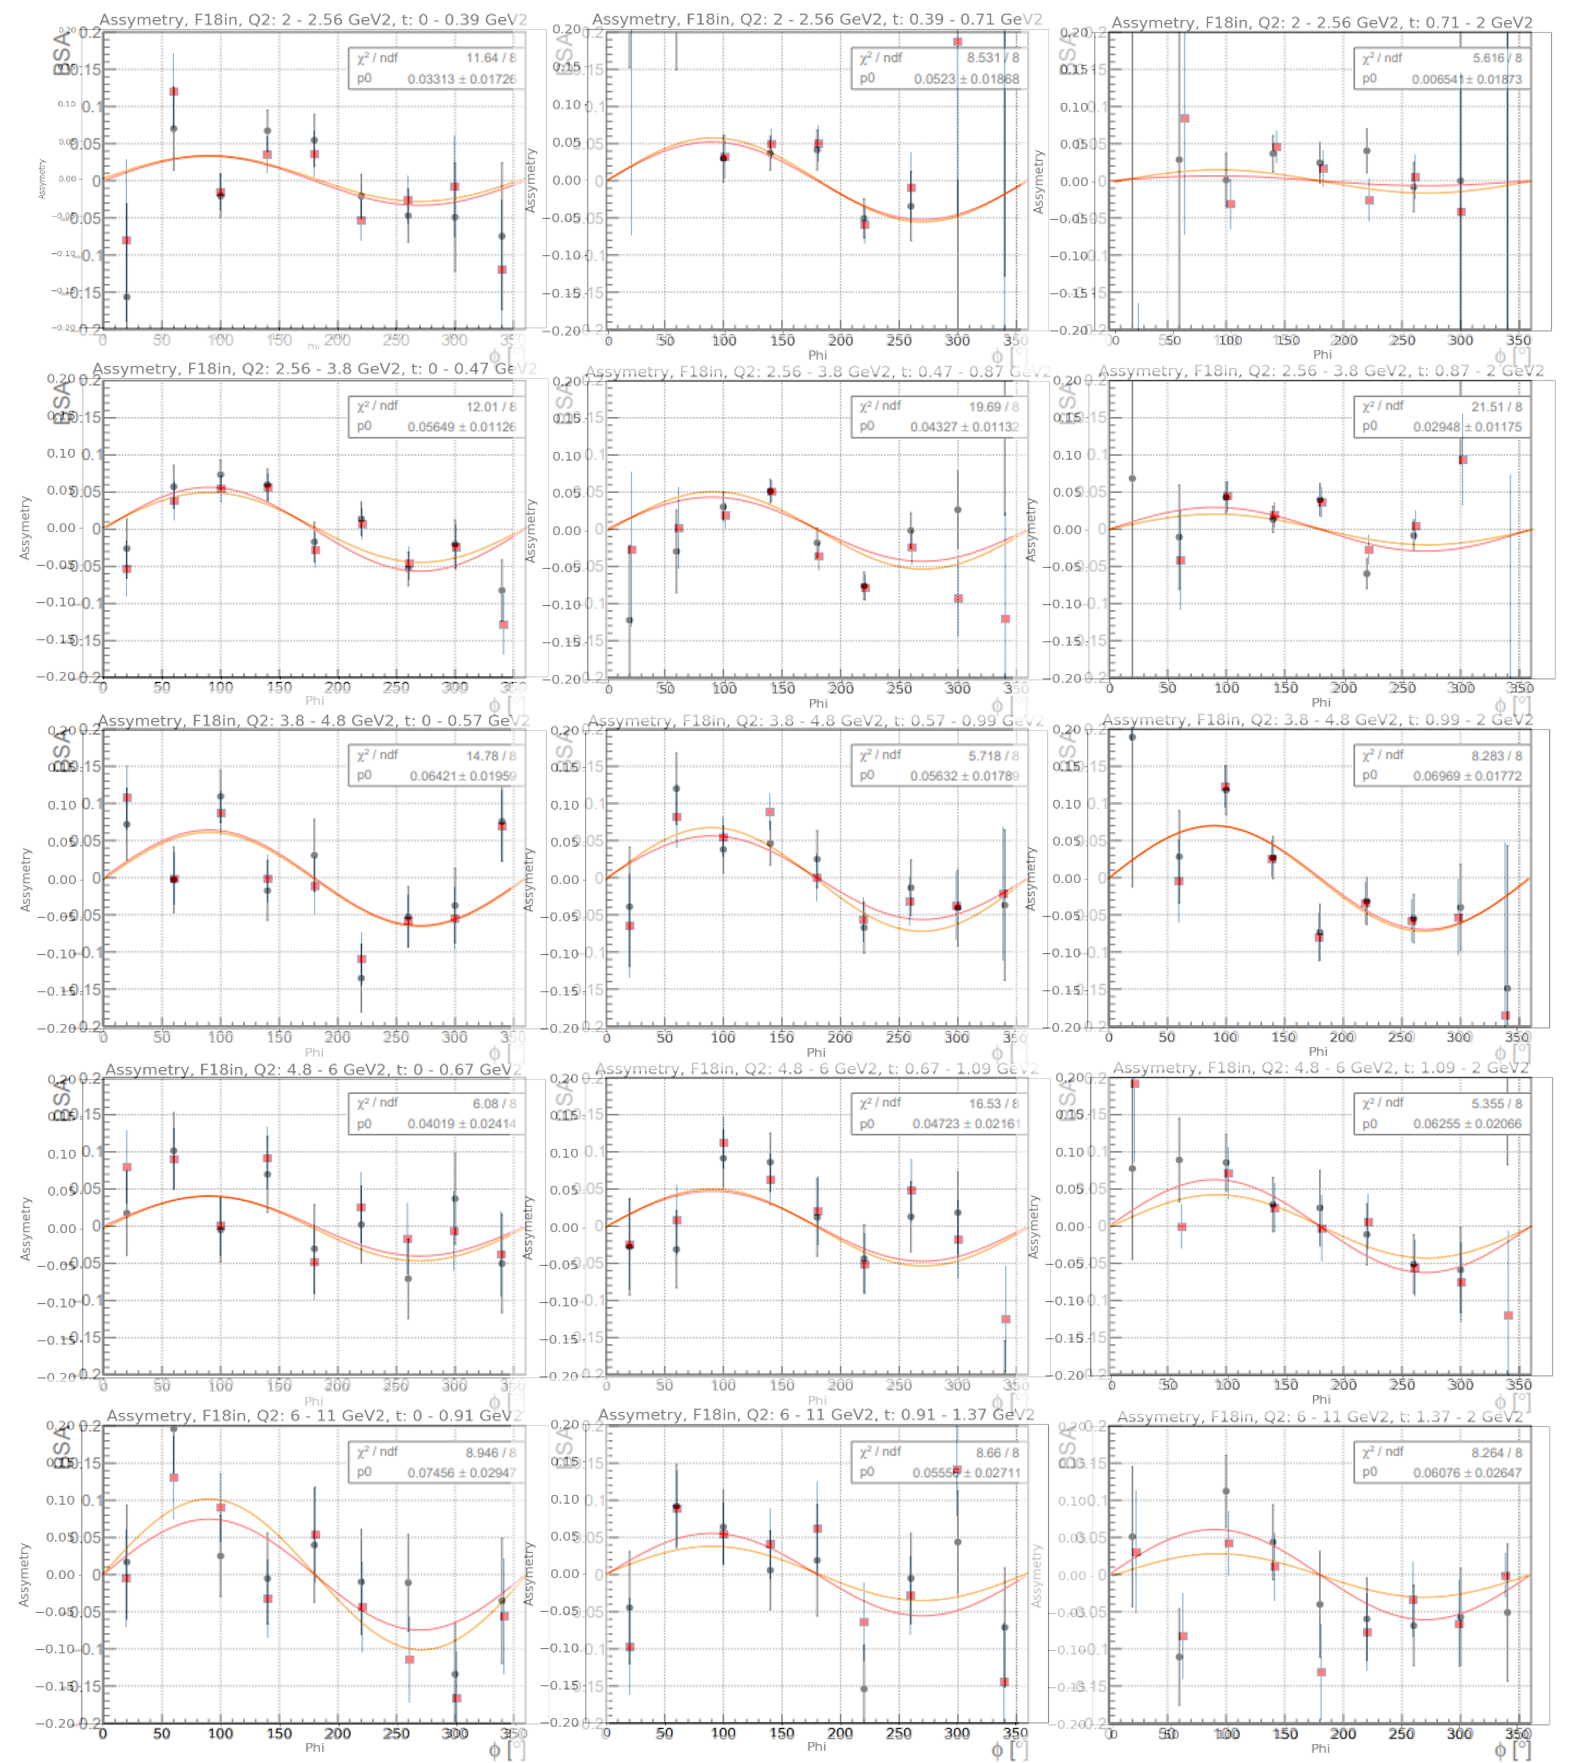
\includegraphics[width=0.75\linewidth]{BSA.png}
	
	
	\caption{Overlay comparison of Andrey Kim's results (black datapoints, red fit line) and Bobby's results (red datapoints, orange fit line).}
	\label{fig:good}
\end{figure}

%\section{Proton PID lookback}
%We extended the analysis to positive tracks.
%Fig.~\ref{fig:finaldatapid} shows the exclusive distributions for positive tracks that were not identified as protons.
%It seems that they are valid exclusive $\pi^0$ electroproduction events even though the positive track was not identified as proton.
%Most of the misidentified tracks happen to be reconstructed in Central Detector.
%Based of Fig.~\ref{fig:finaldatapid} we can make a conclusion that exclusive cuts that we are able to apply because of detection of all final state particles allow us to clean up our sample even without proton PID cuts on positive tracks.
%There seems to be more background for the events with misidentified proton so the tracking improvements (central in particular) would help to clean up the sample in the future.

%\begin{figure}[h]
%    \centering
%    \includegraphics[page=3,width=0.4\linewidth]{figures/eppi0_misc.pdf}
%    \includegraphics[page=4,width=0.4\linewidth]{figures/eppi0_misc.pdf}
%\caption{On the left: is the distribution of $MM^2_{epX}$ for non-proton positive tracks that would pass exclusivity cuts.
%On the right: polar angle for protons in FD (blue), protons in CD (green), non-proton positives in CD (red).}
%    \label{fig:finaldatapid}s
%\end{figure}



%\section{BACKUP}
%\noindent

%\begin{tcolorbox}
%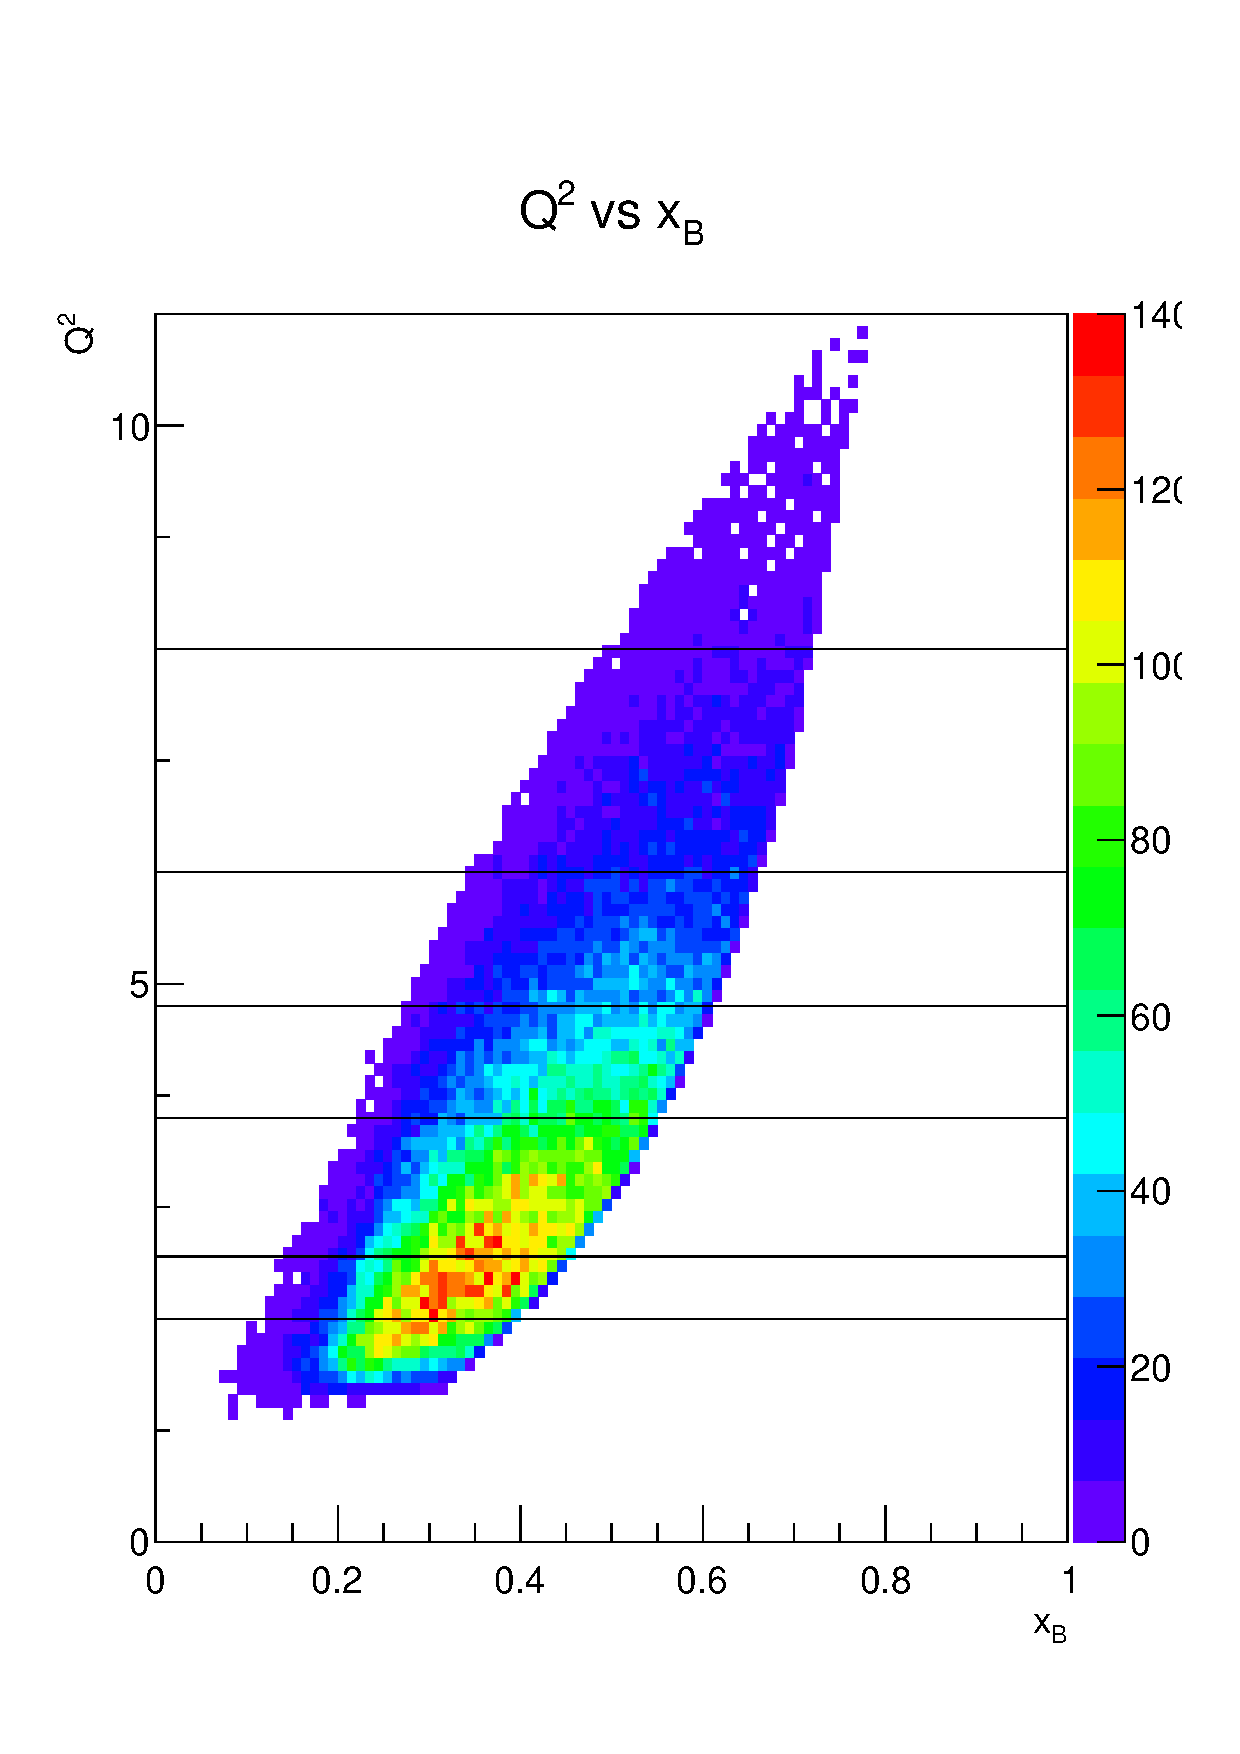
\includegraphics[page=1,width=0.48\linewidth]{figures/bsa_eppi0_ge_pro_fd.pdf}
%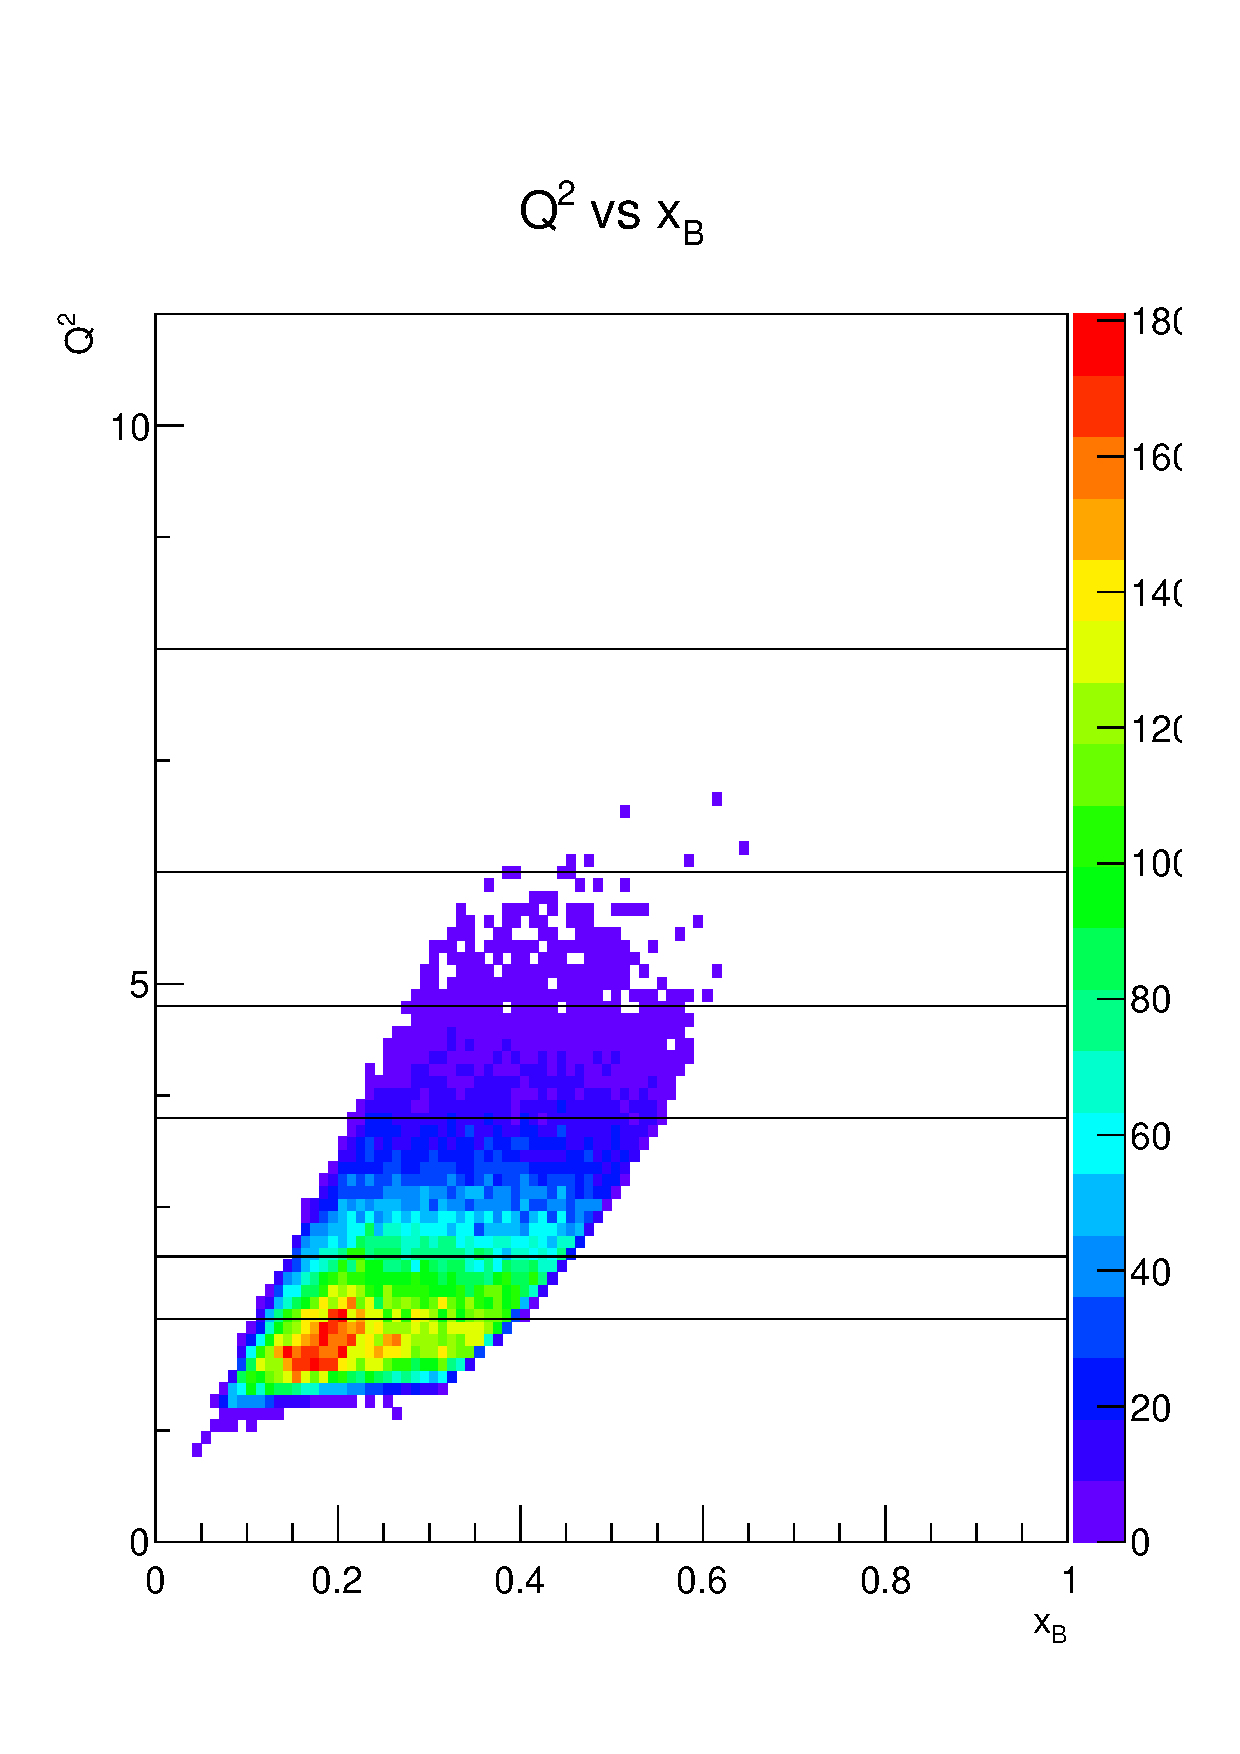
\includegraphics[page=1,width=0.48\linewidth]{figures/bsa_eppi0_ge_pro_cd.pdf}
%\end{tcolorbox}

%\begin{tcolorbox}
%\includegraphics[page=2,width=0.48\linewidth]{figures/bsa_eppi0_ge_pro_fd.pdf}
%\includegraphics[page=2,width=0.48\linewidth]{figures/bsa_eppi0_ge_pro_cd.pdf}
%\end{tcolorbox}

%\begin{tcolorbox}
%\includegraphics[page=3,width=0.48\linewidth]{figures/bsa_eppi0_ge_pro_fd.pdf}
%\includegraphics[page=3,width=0.48\linewidth]{figures/bsa_eppi0_ge_pro_cd.pdf}
%\end{tcolorbox}

%\begin{tcolorbox}
%\includegraphics[page=4,width=0.48\linewidth]{figures/bsa_eppi0_ge_pro_fd.pdf}
%\includegraphics[page=4,width=0.48\linewidth]{figures/bsa_eppi0_ge_pro_cd.pdf}
%\end{tcolorbox}

%\begin{tcolorbox}
%\includegraphics[page=5,width=0.48\linewidth]{figures/bsa_eppi0_ge_pro_fd.pdf}
%\includegraphics[page=5,width=0.48\linewidth]{figures/bsa_eppi0_ge_pro_cd.pdf}
%\end{tcolorbox}

%\begin{tcolorbox}
%\includegraphics[page=6,width=0.48\linewidth]{figures/bsa_eppi0_ge_pro_fd.pdf}
%\includegraphics[page=6,width=0.48\linewidth]{figures/bsa_eppi0_ge_pro_cd.pdf}
%\end{tcolorbox}

%\begin{tcolorbox}
%\includegraphics[page=7,width=0.48\linewidth]{figures/bsa_eppi0_ge_pro_fd.pdf}
%\includegraphics[page=7,width=0.48\linewidth]{figures/bsa_eppi0_ge_pro_cd.pdf}
%\end{tcolorbox}

